\documentclass[11pt]{article}
\usepackage{latexsym}
\usepackage{amsmath}
\usepackage{amssymb}
\usepackage{amsthm}
\usepackage{epsfig}
\usepackage{bbm}
\usepackage[tight]{subfigure}

\usepackage{amsmath}

\DeclareMathOperator*{\minimize}{min}
\DeclareMathOperator*{\maximize}{max}

\usepackage{algorithm}
 %on linux you may need to run sudo apt-get install texlive-full to install algorithm.sys
\usepackage{algorithmic}

\usepackage{verbatim}

\newcommand{\handout}[5]{
  \noindent
  \begin{center}
  \framebox{
    \vbox{
      \hbox to 5.78in { {#1} \hfill #2 }
      \vspace{4mm}
      \hbox to 5.78in { {\Large \hfill #5  \hfill} }
      \vspace{2mm}
      \hbox to 5.78in { {\em #3 \hfill #4} }
    }
  }
  \end{center}
  \vspace*{4mm}
}

\newcommand{\lecture}[5]{\handout{#1}{#2}{#3}{#4}{#5}}
\newcommand{\collision}[0]{\mathrm{collision}}
\newcommand{\nocollision}[0]{\overline{\collision}}

\newcommand*{\QED}{\hfill\ensuremath{\square}}

\newtheorem{theorem}{Theorem}
\newtheorem{corollary}[theorem]{Corollary}
\newtheorem{lemma}[theorem]{Lemma}
\newtheorem{observation}[theorem]{Observation}
\newtheorem{proposition}[theorem]{Proposition}
\newtheorem{definition}[theorem]{Definition}
\newtheorem{claim}[theorem]{Claim}
\newtheorem{fact}[theorem]{Fact}
\newtheorem{assumption}[theorem]{Assumption}
\newtheorem{note}[theorem]{Note}

% 1-inch margins, from fullpage.sty by H.Partl, Version 2, Dec. 15, 1988.
\topmargin 0pt
\advance \topmargin by -\headheight
\advance \topmargin by -\headsep
\textheight 8.9in
\oddsidemargin 0pt
\evensidemargin \oddsidemargin
\marginparwidth 0.5in
\textwidth 6.5in

\parindent 0in
\parskip 1.5ex
%\renewcommand{\baselinestretch}{1.25}

\begin{document}

\lecture{Statistical Techniques in Robotics (16-831, S21)}{Lecture \#18
  (Monday, April 12)}{Lecturer: Kris Kitani}{Scribes: Zach Patterson, Samuel Triest}{Model-Free Value Prediction (Part 2)}

\section{Review}
Last lecture introduced the concept of \underline{model-free value prediction}, or the process of inferring a value function $V(s)$ without access to the underlying MDP (i.e. no $p(s' | s, a)$ or $r(s, a, s')$). In order to compute a value function, we instead use interaction samples from the target environment $\Epsilon$. This extension of the framework is often important when considering systems that act in real-world environments, as it is often impractical/impossible to write down a transition function that perfectly captures the true dynamics of the system.

%This section serves as a review of the previous lecture and any other context required to frame the content of the current lecture. 

%You may format the scribes in any way you like, aside from changing font style, size and page format. Please use subsections and paragraphs to increase the readability of your notes.

%Length requirement 1-2 pages.
\subsection{Problem Setup}
The current problem formulation is as follows:\\\\
\textbf{Goal:} Estimate the value function $v_\pi(s)$ of a policy $\pi$ acting in an environment $\mathcal{E}$  that is ``close'' \footnote{I'm using a vague term here because as mentioned in class, different estimators minimize different measures of closeness (i.e. MSE vs. MLE).} to the true value function  $V_\pi(S)$ of the $\pi$ in $\mathcal{E}$.\\\\
\textbf{Inputs:} We are given the policy $\pi(\cdot | s)$ and a set of $K$ trajectories $\tau$, where $\tau_k$ is defined as follows:

$\tau_k = [(s_1, a_1, r_1, s_2), \hdots (s_{T-1}, a_{T-1}, r_{T-1}, s_T)]$, where:
\begin{itemize}
    \item $s_1 \sim \rho(\cdot)$
    \item $a_t \sim \pi(\cdot|s_t) \forall t$
    \item $r_t \sim r(s_t, a_t, s_{t+1})) \forall t < T$
    \item $s_t \sim p(\cdot | a_{t-1}, s_{t-1}) \forall t > 1$
\end{itemize}
Essentially, we are given k trajectories $\tau$, where each trajectory is comprised of $T$ consecutive interactions in the environment by the policy. Each tuple in the trajectory records how the state changed when the policy took action $a$ in state $s$, and how much reward this transition incurred. Note that $\rho(\cdot)$, $\p(\cdot|a, s)$ and $r(s_t, a_t, s_{t+1})$ are all part of the environment and are not available to our value prediction algorithm. Instead, we must infer (usually implicitly) these distributions from out data $\tau_1 \hdots \tau_k$. This is the major difference between model-based and model-free value prediction.

\subsection{Monte-Carlo Prediction}
In general, in order to perform model-free value prediction, we need to use some estimator of the value function. This estimator will be referred to as $G^{(t)}$. The previous lecture introduced an algorithm that uses an intuitive estimator $G^{(t)}$: the \underline{Monte-Carlo Estimator}. Given a trajectory $\tau$, the Monte-Carlo estimator says that:

\begin{equation}
    G^{(t)} \triangleq \Sigma_{k=t}^{T} \gamma^{k-t} r_k
\end{equation}
Simply put, the Monte-Carlo estimator says that we can estimate $V_\pi(s)$ as our observed return from state $s$. Using this estimator, we can derive several algorithms for model-free value prediction, with the most straightforward being every-visit MC prediction, presented in Algorithm \ref{algo:every_visit_mc}. 

\begin{algorithm}[H]
\caption{Every-Visit MC Prdiction}
\label{algo:every_visit_mc}
\begin{algorithmic}[1]
\STATE $V(s) \leftarrow k \;\; \forall s \in \mathcal{S}$ \hfill $\triangleright$ Initialize the value function to some arbitrary value.
\FOR{$1\;\hdots\;K$}
    \STATE $\tau_k \sim \pi, \mathcal{E}$ \hfill $\triangleright$ Sample a trajectory by rolling out the policy in the environment.
    \STATE ${s_t, a_t, r_t, s_{t+1}} \sim \tau_k$ \hfill $\triangleright$ Decompose trajectory into transitions.
    
    \FOR{$t \in 0 \hdots T$}
        \STATE $G^{(t)} = \Sigma_{i=t}^T \gamma^{i-t} r_i$ \hfill $\triangleright$ Estimate $V$ as reward-to-go from current state
        \STATE $V(s_t) \leftarrow V(s_t) + \alpha (G^{(t)} - V(s_t))$ \hfill $\triangleright$ Update $V$ by taking a step towards the estimator $G^{(t)}$
    \ENDFOR
    
\ENDFOR
\end{algorithmic}
\end{algorithm}
One interesting thing to note is that this algorithm can be considered as a form of online gradient descent (see line 7), where the objective function that we are trying to minimize is:
\begin{equation}
    J(\theta) = \frac{\alpha}{2} (G^{(t)} - V(s_t))^2
\end{equation}
We can observe that this is simply a scaled version of the MSE between our value function and our value estimator. This algorithm has several properties that will be discussed later in these notes, as to directly compare them with TD Prediction.

\section{Summary}
\subsection{Temporal Difference (TD) Prediction}
Outline: Derive estimator from Bellman eq. Talk about 1-step vs. n-step. Mention MC as TD-inf. Give 1 step vs. n-step algo. Discuss tradeoffs: bias/variance. Usability online. MSE vs. MLe (cite the Sutton paper). Segway: What is optimal n?

Using the recursive definition of the V function as:
\begin{equation}
    V_\pi(s) = \mathop{\mathbb{E}}_{a \sim \pi(\cdot|s), s' \sim p(\cdot | a, s)}[r(s, a, s') + \gamma V_\pi(s')]
\end{equation}
we can derive another family of potentially useful estimators of $V_\pi$. Since the data we've collected can be assumed to come from the policy $\pi$ and dynamics $p$, we can construct an estimator:
\begin{equation}
    G^{(t)} \triangleq r_t + \gamma V_\pi(s_{t+1})
\end{equation}
This estimator is known as the \underline{TD(0) estimator}, or the \underline{1-step TD Estimator}. The recursive nature of the Bellman equation lets us derive a family of estimators known as \underline{n-step TD estimators}, where the n-step TD estimator $G^{(t)}(n)$ is:
\begin{equation}
    G^{(t)}(n) \triangleq \sum_{k=t}^{t+n} [\gamma^{k-t} r_{k}] + \gamma^n V_\pi(s_{t+n})
\end{equation}
In general, the TD estimators utilize a technique called \underline{bootstrapping}, which refers to how the definition of the estimator for a given state requires using the estimator on other states (with the base case being at terminal states).\\\\
Another interesting fact is that the Monte-Carlo estimator is equal to the $\infty$-step TD estimator. This follows from the fact that $\gamma^\infty = 0, \forall \gamma \in [0, 1)$. As such, we are left with the discounted sum of rewards for all timesteps (which is just the Monte-Carlo estimator).\\\\

Below are the algorithms for model-free value prediction using the 1-step and n-step TD estimators.

\begin{algorithm}[H]
\caption{1-Step TD Prediction}
\label{algo:1step_td}
\begin{algorithmic}[1]
\STATE $V(s) \leftarrow k \;\; \forall s \in \mathcal{S}$ \hfill $\triangleright$ Initialize the value function to some arbitrary value.
\FOR{$1\;\hdots\;K$}
    \STATE $\tau_k \sim \pi, \mathcal{E}$ \hfill $\triangleright$ Sample a trajectory by rolling out the policy in the environment.
    \STATE ${s_t, a_t, r_t, s_{t+1}} \sim \tau_k$ \hfill $\triangleright$ Decompose trajectory into transitions.
    
    \FOR{$t \in 0 \hdots T-1$}
        \STATE $G^{(t)} = r_t + \gamma V(s_{t+1})$ \hfill $\triangleright$ Estimate $V$ using 1-step TD.
        \STATE $V(s_t) \leftarrow V(s_t) + \alpha (G^{(t)} - V(s_t))$ \hfill $\triangleright$ Update $V$ by taking a step towards the estimator $G^{(t)}$
    \ENDFOR
    \STATE $G^{(T)} = r_T$ \hfill $\triangleright$ Handle the final state.
    \STATE $V(s_T) \leftarrow V(s_T) + \alpha (G^{(T)} - V(s_T))$
\ENDFOR
\end{algorithmic}
\end{algorithm}

\begin{algorithm}[H]
\caption{n-Step TD Prediction}
\label{algo:nstep_td}
\begin{algorithmic}[1]
\STATE $V(s) \leftarrow k \;\; \forall s \in \mathcal{S}$ \hfill $\triangleright$ Initialize the value function to some arbitrary value.
\FOR{$1\;\hdots\;K$}
    \STATE $\tau_k \sim \pi, \mathcal{E}$ \hfill $\triangleright$ Sample a trajectory by rolling out the policy in the environment.
    \STATE ${s_t, a_t, r_t, s_{t+1}} \sim \tau_k$ \hfill $\triangleright$ Decompose trajectory into transitions.
    
    \FOR{$t \in 0 \hdots T-n$}
        \STATE $G^{(t)} = \sum_{i=t}^{t+n} [\gamma^{i-t} r_{i}] + \gamma^n V(s_{t+n})$ \hfill $\triangleright$ Estimate $V$ using n-step TD.
        \STATE $V(s_t) \leftarrow V(s_t) + \alpha (G^{(t)} - V(s_t))$ \hfill $\triangleright$ Update $V$ by taking a step towards the estimator $G^{(t)}$
    \ENDFOR
     \FOR{$t \in (T-n+1) \hdots T$}
        \STATE $G^{(t)} = \sum_{i=t}^{T} [\gamma^{i-t} r_{i}] + \gamma^{T-n} V(s_{T})$ \hfill $\triangleright$ Handle the last n states.
        \STATE $V(s_t) \leftarrow V(s_t) + \alpha (G^{(t)} - V(s_t))$
    \ENDFOR
\ENDFOR
\end{algorithmic}
\end{algorithm}
As mentioned, there are several tradeoffs between TD estimators and Monte-Carlo estimators. Some important tradeoffs to consider are:
\begin{enumerate}
    \item Usability Online
    \item Bias/Variance Tradeoff
\end{enumerate}
The following subsections will discuss the tradeoffs between the Monte-Carlo estimator and the 1-step TD estimator as they present extreme points on the tradeoff spectrum, with the n-step TD estimators falling some place in the middle.

\subsubsection{Usability Online}
One major distinction between the Monte-Carlo estimator and the 1-step TD estimator is that we cannot use the Monte-Carlo estimator in an online fashion. Recall the Monte-Carlo estimator:
\begin{equation*}
    G^{(t)} \triangleq \Sigma_{k=t}^{T} \gamma^{k-t} r_k
\end{equation*}
As we can see, in order to get the estimate at time $t$, we require the reward at the final timestep $T$. This is not the case for the 1-step (and n-step) TD estimator:
\begin{equation*}
    G^{(t)} \triangleq r_t + \gamma V_\pi(s_{t+1})
\end{equation*}
where we only require the reward at the current timestep and the next state (for n-step TD, we need the next n rewards and the state at $t_n$). 

\subsubsection{Bias/Variance Tradeoff}
The Monte-Carlo estimator and 1-step TD estimator have a very significant tradeoff between their bias and variance. In general, the Monte-Carlo estimator has high variance but no bias, while the 1-step TD estimator has low variance but nonzero bias. Recall that the definition of bias of an estimator $G$ of a quantity x is:
\begin{equation}
    B(G) = \mathbb{E}[G] - x
\end{equation}
For our case, the quantity that we try to measure is $v_\pi(s) = \mathop{\mathbb{E}}_{\tau \sim \pi, \mathcal{E}}[\sum_t \gamma^t r_t]$ (using lowercase to indicate that this is the true value function and not our estimator $V_\pi(s)$). Clearly, the Monte-Carlo estimator is unbiased:
\begin{equation}
    B(G_{MC}) =\mathop{\mathbb{E}}_{\tau \sim \pi, \mathcal{E}}[\sum_t \gamma^t r_t] -  \mathop{\mathbb{E}}_{\tau \sim \pi, \mathcal{E}}[\sum_t \gamma^t r_t] = 0
\end{equation}
However, the bias of the 1-step TD-estimator is not necessarily 0.
\begin{equation}
    B(G_{TD}) =\mathop{\mathbb{E}}_{\tau \sim \pi, \mathcal{E}}[r_t + \gamma V(s_{t+1})] -  \mathop{\mathbb{E}}_{\tau \sim \pi, \mathcal{E}}[\sum_t \gamma^t r_t] = \mathop{\mathbb{E}}_{\tau \sim \pi, \mathcal{E}}[\gamma V(s_{t+1}) - \sum_{i=t+1}^T \gamma^i r_i]
\end{equation}
Note that this $V$ in the bias is not the true $v$ and can take an arbitrary value depending on its initialization. \\\\
On the other hand, the Monte-Carlo estimator has much higher variance due to the fact that it contains many more terms, which each have variance.\\\\
Overall, the decision on whether to use Monte-Carlo estimates or TD estimates is problem-specific. However, the authors note that TD estimation seems to be more popular, as can be observed by its use to estimate value functions in many seminal papers in RL in recent years. \cite{mnih2013playing, mnih2016asynchronous, lillicrap2015continuous, fujimoto2018addressing, haarnoja2018soft} all use 1-step TD to train a neural network estimator of either the $V$ or $Q$ function, and \cite{hessel2018rainbow} uses an n-step TD estimator.

\subsection{TD-$\lambda$}
\subsubsection{Offline- $\lambda$-Return}
At the end of the last section, we saw that the success of the TD algorithm is dependent on the number of steps ahead used in the estimate (N). In this section, we'll discuss an algorithm that allows us to avoid specifying N. At the heart of this approach, called TD($\lambda$), is the realization that we can combine multiple estimates to form a TD Target, for example:
\begin{equation}
    G^{(t)} = \frac{1}{3}G^{(t)}(3)+\frac{1}{3}G^{(t)}(5)\frac{1}{3}G^{(t)}(7).
\end{equation}

So what if we combine the targets for all N? This gives us the infinite horizon $\lambda$-Return:
\begin{equation}
    G_\lambda^{(t)} = (1 - \lambda) \sum_{n=1}^\infty \lambda^{n-1} G^{t}(n), \lambda \in [0,1].
\end{equation}

$\lambda$, called the trace decay factor, provides a weighting scheme in which the longer estimates (higher n) are given less weight. See \ref{fig:decay} for a depiction of this effect.

\begin{figure}
    \centering
    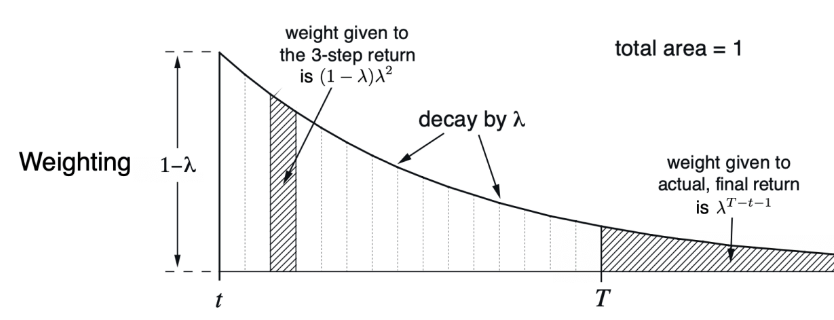
\includegraphics[width=0.8\textwidth]{images/lambda decay.png}
    \caption{Shows the decay of the $\lambda$-Return with increasing steps \cite{sutton2018reinforcement}.}
    \label{fig:decay}
\end{figure}

In practice, we must truncate the return to a finite horizon case:

\begin{equation}
    G_\lambda^{(t)} = (1 - \lambda) \sum_{n=1}^{T - t - 1} \lambda^{n-1} G^{t}(n) + \lambda^{T - t - 1} G^{t}({T - t - 1}), \lambda \in [0,1].
\end{equation}

Looking at a few special cases, we see that when $\lambda = 1$, $G_\lambda^{(t)} = G^{t}(T - t - 1)$, which is the Monte Carlo estimate. When $\lambda = 0$, $G_\lambda^{(t)} = G^{t}(1)$, which is the one step TD estimate. The following shows the Offline-$\lambda$-Return algorithm:

\begin{algorithm}[H]
\caption{Offline-$\lambda$-Return($\pi,\alpha, \lambda$)}
\label{algo:every_visit_mc}
\begin{algorithmic}[1]
\FOR{$1\;\hdots\;E$}
    \STATE $\{s^{(t)},a^{(t)}, r^{(t)}\}_{t=0}^T \sim \mathcal{E}|\pi$ \hfill $\triangleright$ Sample a full episode.
    
    \FOR{$t \in 0 \ddots T$}
        \STATE $G_\lambda^{(t)} \leftarrow (1-\lambda)\sum_{n=1}^\infty \lambda^{n-1} G^{(t)}(n)$ \hfill $\triangleright$ Precompute all returns.
    \ENDFOR
     \FOR{$t \in 0 \ddots T$}
        \STATE $V(s^{(t)}) \leftarrow V(s^{(t)}) + \alpha[G_\lambda^{(t)} - V(s^{(t)})]$ \hfill $\triangleright$ Precompute all returns.
    \ENDFOR
    
\ENDFOR
\end{algorithmic}
\end{algorithm}

\begin{figure}
    \centering
    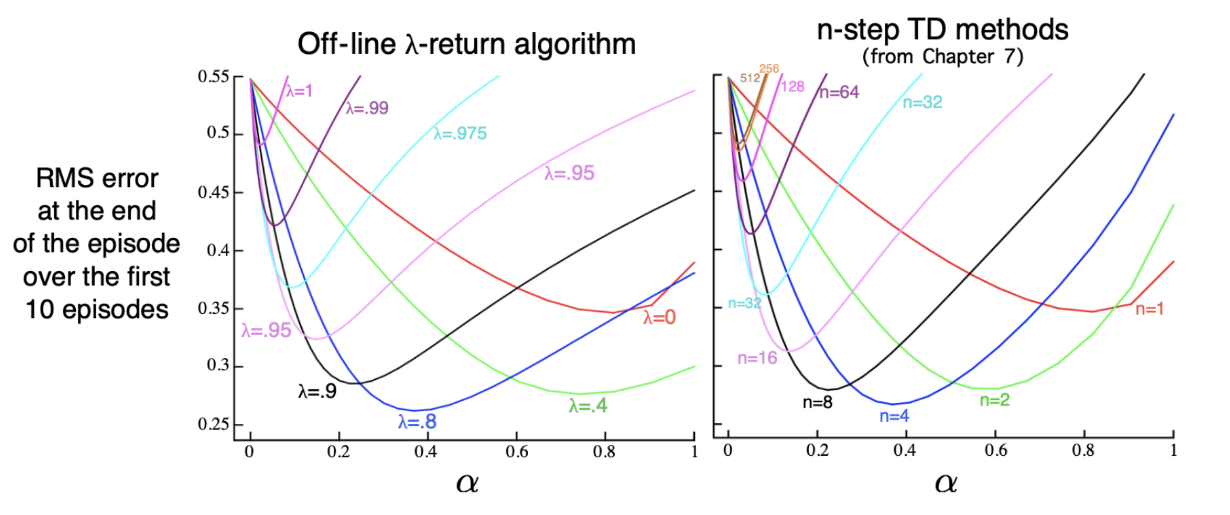
\includegraphics[width=\textwidth]{images/lam performance comparison.png}
    \caption{Shows the performance of Offline-$\lambda$-Return versus the n-step TD \cite{sutton2018reinforcement}.}
    \label{fig:comp}
\end{figure}

Figure \ref{fig:comp} shows that the offline lambda return algorithm is only a bit better than the n-step TD approach so why would we use it? The answer is that this algorithm provides a tool for understanding $\lambda$-returns but it is not a practical algorithm because you need to access the full future trajectory to update the value function (impossible online). However, the 'backwards TD($\lambda$) perspective' is useful for the practical implementation, which uses the concept of eligibility traces.

\subsubsection{Eligibility Returns}
The TD($\lambda$) update can be written as a sum of weighted one step TD errors:
\begin{equation}
    \Delta V(s^t) = G_\lambda^{(t)} - V(s^t) = \sum_{i=0}^\infty(\gamma \lambda)^i \delta^{(t+i)}
\end{equation}
\begin{equation}
    \delta^{(t)} = r{(t)}+ \gamma V(s^{(t+1)}) - V(s^{(t)}).
\end{equation}

It's important to note that $\lambda$ and $\gamma$ are not subsumed into the same discount factor because they will eventually come to have independent effects on the function. The above is easy to prove algebraically by plugging in the definition of $\lambda$-return, expanding the sum, separating out the n-step TD targets, and canceling terms. 

We can equivalently write the update as a decaying weighted sum of future TD errors at time k:
\begin{equation}
    \Delta V(s^{(k)} = s) = \sum_{i=0}^\infty(\gamma \lambda)^i \delta^{(k+i)} = \sum_{t=k}^\infty(\gamma \lambda)^{t-k} \delta^{(t)}.
\end{equation}

We can now rewrite this as:
\begin{equation}
    \Delta V(s^{(k)} = s) = \sum_{t=k}^\infty(\gamma \lambda)^{t-k} \delta^{(t)} = \sum_{t=1}^{k-1}(0)\delta^{(t)} + \sum_{t=k}^\infty(\gamma \lambda)^{t-k} \delta^{(t)} = \sum_{t=1}^\infty z^{(t)}(s) \delta^{(t)}
\end{equation}
where 
\begin{equation}
z^{(t)}(s) = \begin{cases}
    0 & t<k \\
    (\gamma \lambda)^{t-k} & t \geq k.
    \end{cases}
\end{equation}

This new value function update expression contains the weight/credit function $z$ within the infinite horizon sum, giving no weight to the past and a decaying weight to the future. This weighting/credit function is called the eligibility trace. \\
Therefore, the eligibility trace is 0 prior to the occurrence of some state s at k. When t=k, the eligibility trace is 1 and it decays after time k with time.\\
The eligibility trace can also be written as an incremental update:
\begin{equation}
    z^{(t)}(s) = \gamma \lambda z^{(t-1)}(s) + \mathbbm{1}[s^{(t)}=s].
\end{equation}

This form is slightly different than the previous form in that every time it sees state s, 1 is added (as opposed to being set to 1 when seeing state s). Then the function decays according to the same discount factor and trace decay factor as before. This gives additional weight to frequency as well as the to recency. See Figure \ref{fig:eligib} for a depiction of this function.

\begin{figure}
    \centering
    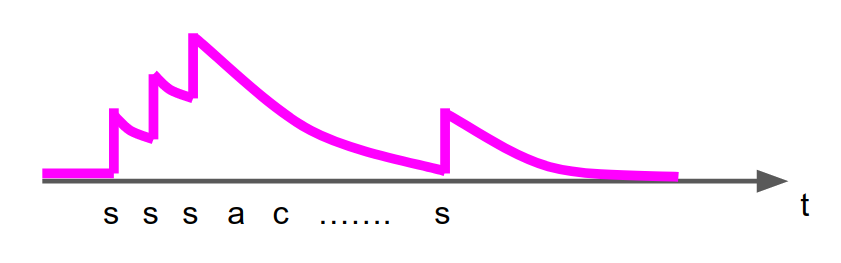
\includegraphics[width=0.8\textwidth]{images/eligibility.png}
    \caption{The eligibility trace over time. The x axis is time. Note that states are written when they occur as letters. In this case, we're tracking the eligibility trace of state s.}
    \label{fig:eligib}
\end{figure}

%\section*{References}
%Include your references here. Please cite any resources you found useful.	
%Populate the refs.bib file or list your references manually. Be consistent in formatting!
{
\bibliography{refs}
\bibliographystyle{unsrt}
}


%This section provides any relevant background material that was not covered in the lectures, but was found to be useful for understanding the material. 
%For example, derivations, theory underlying techniques employed, etc. 

%Additionally, this section can summarizes applications or extensions of these techniques found in the literature. 

\end{document} % Done!


